\documentclass[t]{beamer}
\usetheme{Copenhagen}
\setbeamertemplate{headline}{} % remove toc from headers
\beamertemplatenavigationsymbolsempty

\usepackage{amsmath, array, tikz, tcolorbox, bm, tkz-euclide, pgfplots, graphicx}
\pgfplotsset{compat = 1.16}
\usetkzobj{all}
\everymath{\displaystyle}

\title{Circles}
\author{}
\date{}

\AtBeginSection[]
{
  \begin{frame}
    \frametitle{Objectives}
    \tableofcontents[currentsection]
  \end{frame}
}

\begin{document}

\begin{frame} 
\maketitle
\end{frame}

\begin{frame}[c]
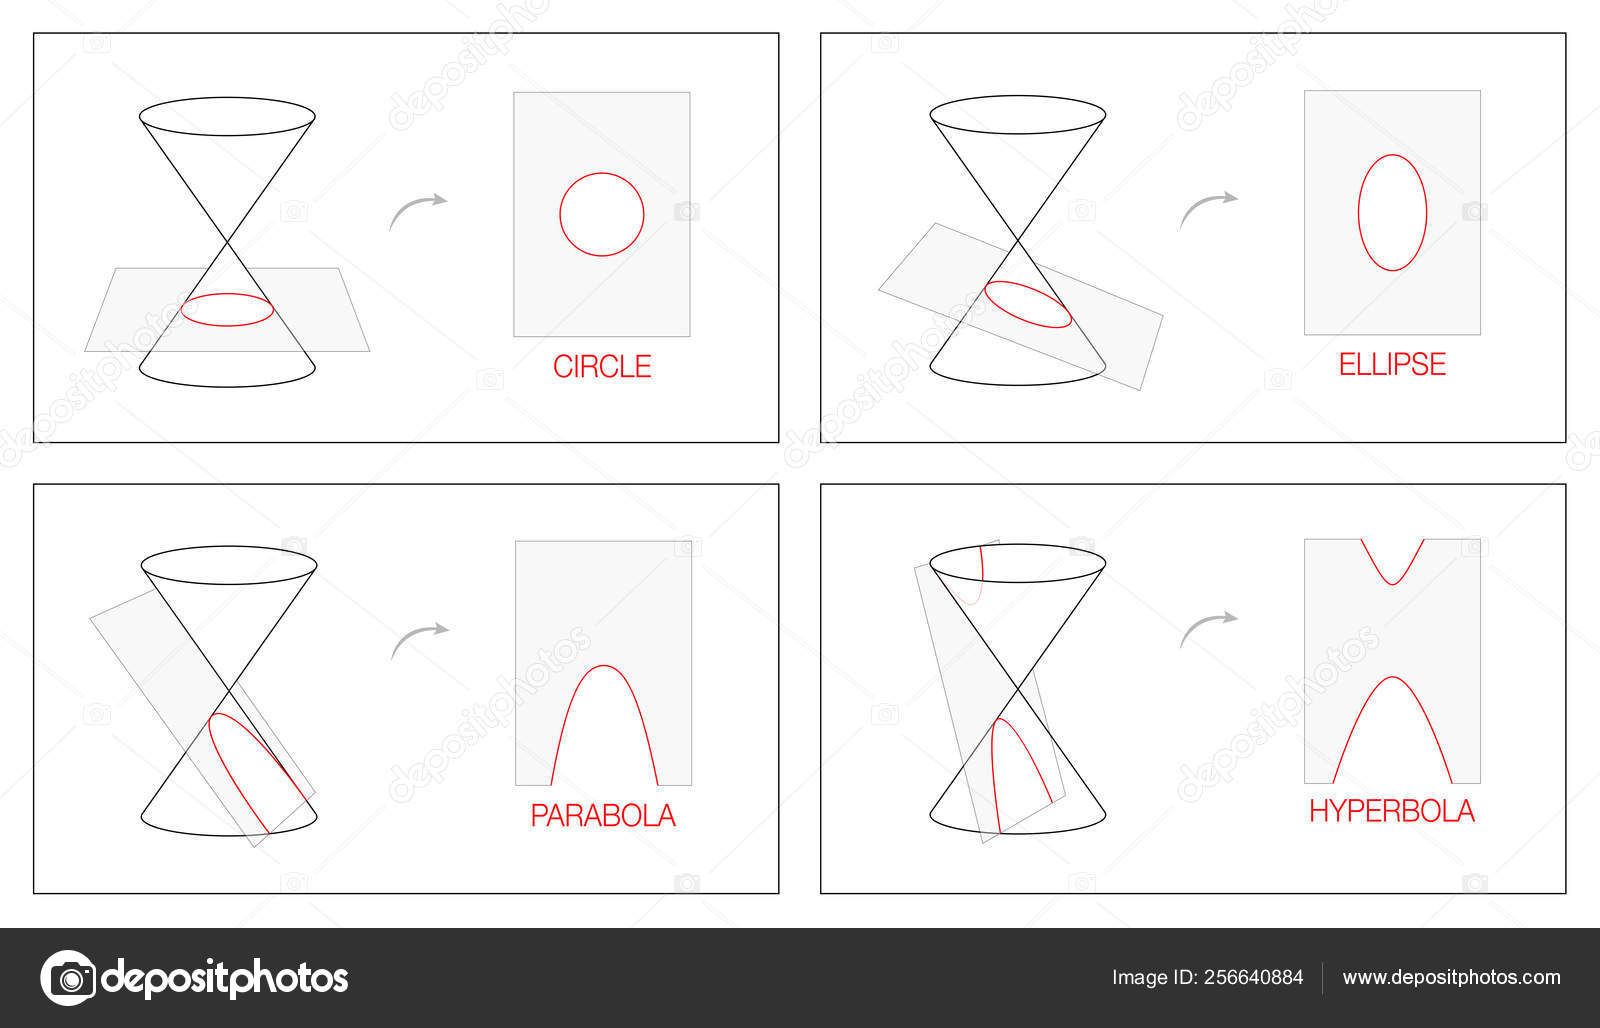
\includegraphics[scale=0.80]{Images/conics.jpg}
\end{frame}

\section{Identify the center and radius of a circle.}

\begin{frame}{Circles}
You may remember circles from geometry class. In this chapter, we will look at equations and properties of circles. \newline\\	\pause

\begin{tcolorbox}[colback=red!10!white, colframe=red!60!black,, title=\textbf{Circles}]
The set of points, each of whose distance from a fixed point (the center) is the same.
\end{tcolorbox}
\vspace{11pt}	\pause

The standard form of the equation of a circle is 
\[
(x-h)^2+(y-k)^2 = r^2
\]

with center $(h, \, k)$ and radius $r$. 
\end{frame}

\begin{frame}{Example 1}
Identify the center and exact radius of each.	\newline\\
(a)	\quad	$(x-4)^2 + (y+3)^2 = 49$	\newline\\
\onslide<2->{Center: $(4, -3)$}	\newline\\
\onslide<3->{Radius: $\sqrt{49}$ }	\onslide<4->{$=7$}
\end{frame}

\begin{frame}{Example 1}
(b)	\quad	$(x+1)^2 + (y-7)^2 = 72$	\newline\\
\onslide<2->{Center: $(-1, 7)$}	\newline\\
\onslide<3->{Radius: $\sqrt{72}$ } \onslide<4->{$=6\sqrt{2}$}
\end{frame}

\begin{frame}{Writing the Standard Form of the Equation of a Circle}

To get the standard form, perform the following steps:	\newline\\	
\begin{enumerate}
    \item Bring the constant over to the other side of the equation.	\newline\\ \pause
    \item Find the vertex of the $x$-terms and $y$-terms. \newline\\ \pause
        \begin{itemize}
            \item The $x$-coordinates of each vertex will represent $h$ and $k$, respectively.	\newline\\ \pause
            \item The absolute value $y$-coordinates will be added to the constant.
        \end{itemize}
\end{enumerate}
\end{frame}

\begin{frame}{Example 2}
Identify the center and exact radius of each.	\newline\\
(a)	\quad	$x^2-4x+y^2+6y-23=0$	
\onslide<2->{\[{\color{blue}\bm{x^2 - 4x}} \qquad + {\color{red}\bm{y^2 - 6y}} \qquad = 23\]} 
\onslide<3->{{\color{blue}\textbf{Vertex: }$\bm{(2,-4)}$}}	\newline\\
\onslide<4->{{\color{red}\textbf{Vertex: }$\bm{(3,-9)}$}}	
\onslide<5->{\[(x-2)^2 + (y-3)^2 = 23 + |-4| + |-9|\]}	
\onslide<6->{\[(x-2)^2+(y-3)^2=36\]}	\\
\onslide<7->{Center: $(2,3)$ \quad Radius: 6}
\end{frame}

\begin{frame}{Example 2}
(b)	\quad $x^2+16x+y^2-8y-1=0$
\onslide<2->{\[{\color{blue}\bm{x^2 + 16x}} \qquad + {\color{red}\bm{y^2 - 8y}} \qquad = 1\]} 
\onslide<3->{{\color{blue}\textbf{Vertex: }$\bm{(-8,-64)}$}}	\newline\\
\onslide<4->{{\color{red}\textbf{Vertex: }$\bm{(4,-16)}$}}	
\onslide<5->{\[(x+8)^2 + (y-4)^2 = 1 + |-64| + |-16|\]}	
\onslide<6->{\[(x+8)^2+(y-4)^2=81\]}	\\
\onslide<7->{Center: $(-8,4)$ \quad Radius: 9}
\end{frame}

\begin{frame}{Example 2}
(c)	\quad $x^2-10x+y^2+2y+14=0$	\newline\\
\onslide<2->{$x^2-10x+y^2+2y=-14$}
\onslide<3->{\[{\color{blue}\bm{x^2 - 10x}} \qquad + {\color{red}\bm{y^2 + 2y}} \qquad = 1\]} 
\onslide<4->{{\color{blue}\textbf{Vertex: }$\bm{(5,-25)}$}}	\newline\\
\onslide<5->{{\color{red}\textbf{Vertex: }$\bm{(-1,-1)}$}}	
\onslide<6->{\[(x-5)^2 + (y+1)^2 = 14 + |-25| + |-1|\]}	
\onslide<7->{\[(x-5)^2+(y+1)^2=40\]}	\\
\onslide<8->{Center: $(5,-1)$ \quad Radius: $2\sqrt{10}$}
\end{frame}

\section{Write the general form of the equation of a circle in standard form}

\begin{frame}{General Form}
Circles can also be written in general form. General form is standard form multiplied out and simplified.    \newline\\	\pause 

General form will have all terms on one side of the equation and 0 on the other.
\end{frame}

\begin{frame}{Example 3}
Write the general form of each of the following.	\newline\\
(a)	\quad $(x-3)^2+y^2=6$
\begin{align*}
\onslide<2->{(x-3)^2 + y^2 &= 6} \\[6pt]
\onslide<3->{x^2 - 6x + 9 + y^2 &= 6} \\[6pt]
\onslide<4->{x^2 - 6x + y^2 + 3 &= 0}
\end{align*}
\end{frame}

\begin{frame}{Example 3}
(b)	\quad $(x+7)^2+(y-5)^2=18$
\begin{align*}
\onslide<2->{(x+7)^2+(y-5)^2 &= 18} \\[6pt]
\onslide<3->{x^2 + 14x + 49 + y^2 - 10y + 25 &= 10} \\[6pt]
\onslide<4->{x^2 + 14x + y^2 - 10y + 74 &= 10} \\[6pt]
\onslide<5->{x^2 + 14x + y^2 - 10y + 64 &= 0}
\end{align*}
\end{frame}


\end{document}